\documentclass[11pt,reqno,twoside]{article}
%>>>>>>> RENAME CURRENT FILE TO MATCH LECTURE NUMBER
% E.g., "lecture_01.tex"

%>>>>>>> DO NOT EDIT MACRO FILE

% >>>> DO NOT EDIT THIS FILE
% If you *must* add or change a macro, please email fkoh@caltech.edu

%=================================================
% Basics
%=================================================

\usepackage{fixltx2e} % Makes \( \) equation style robust, among other
                      % things. Must be the first package.


% Makes ligatured fonts searchable and copyable in pdf readers
\usepackage{cmap} % Load before fontenc 

% Always include these font encodings in your document 
% unless you have a very good reason.
\usepackage[T1]{fontenc}
\usepackage[utf8]{inputenc}

\usepackage{verbatim}

%=====================================
% Look & feel
%=====================================

% Allows for manual space setting
\usepackage{setspace}

%=============
% Fonts
%=============

\usepackage{lmodern} % Improved version of computer modern
\usepackage[scale=0.88]{tgheros} % Helvetica clone for sans serif font


\newcommand\hmmax{2} % Default is 3.
\newcommand\bmmax{2} % Default is 4.

\usepackage{bm} % boldmath must be called after the package
\providecommand{\mathbold}[1]{\bm{#1}}

%=============
% AMS Packages and fonts
%=============
\usepackage{amsmath,amsbsy,amsgen,amscd,amsthm,amsfonts,amssymb} 

%=============
% Margins and paper size
%=============
\usepackage[centering,top=1.5in,bottom=1.2in,left=1.4in,right=1.4in]{geometry}

%=============
% Title setup
%=============
\usepackage{titling}
%\usepackage{nopageno}
\setlength{\droptitle}{-7.5em}

\pretitle{\noindent\rule{0.85\linewidth}{0.2mm}\par%
  \begin{raggedright}\LARGE\sffamily}
\posttitle{\par\end{raggedright}%
\noindent%
\rule{0.85\linewidth}{0.5mm}\par}

\preauthor{\noindent\vspace{0.5em}%
  \sffamily\begin{tabular}[t]{ll}}
  \postauthor{\end{tabular}\par\thispagestyle{plain}}

\predate{\noindent%
  \small\sffamily\itshape\begin{tabular}[t]{l}%
    ACM 256, Winter 2019 \\ %
    Dr.\ Franca Hoffmann \\ %
  }
  \postdate{
  \end{tabular}\par}

%=============
% Section headings
%=============
\usepackage[sf,bf,compact]{titlesec}

%=============
% Tables and lists
%=============
\usepackage{booktabs,longtable,tabu} % Nice tables
\setlength{\tabulinesep}{1mm}
\usepackage[font=small,margin=10pt,labelfont={sf,bf},labelsep={space}]{caption}


\usepackage{enumitem}
\setitemize{itemsep=0pt} 
\setenumerate{itemsep=0pt}
\setlist{labelindent=\parindent,%  % Recommended by enumitem package
  font=\sffamily}


%=============
% Hyperlink colors
%=============
\usepackage[usenames,dvipsnames]{xcolor}
\definecolor{dark-gray}{gray}{0.3}
\definecolor{dkgray}{rgb}{.4,.4,.4}
\definecolor{dkblue}{rgb}{0,0,.5}
\definecolor{medblue}{rgb}{0,0,.75}
\definecolor{rust}{rgb}{0.5,0.1,0.1}

\usepackage{url}
\usepackage[colorlinks=true]{hyperref}
\hypersetup{linkcolor=dkblue}    
\hypersetup{citecolor=rust}      
\hypersetup{urlcolor=rust}     

%=============
% Microtype
%=============
\usepackage[final]{microtype} 

%=============
% Theorems, etc.
%=============
\newtheoremstyle{myThm} % name
    {\topsep}                    % Space above
    {\topsep}                    % Space below
    {\itshape}                   % Body font
    {}                           % Indent amount
    {\sffamily\bfseries}                   % Theorem head font
    {.}                          % Punctuation after theorem head
    {.5em}                       % Space after theorem head
    {}  % Theorem head spec (can be left empty, meaning ‘normal’)

\newtheoremstyle{myRem} % name
    {\topsep}                    % Space above
    {\topsep}                    % Space below
    {}                   % Body font
    {}                           % Indent amount
    {\sffamily}                   % Theorem head font
    {.}                          % Punctuation after theorem head
    {.5em}                       % Space after theorem head
    {}  % Theorem head spec (can be left empty, meaning ‘normal’)

\newtheoremstyle{myDef} % name
    {\topsep}                    % Space above
    {\topsep}                    % Space below
    {}                   % Body font
    {}                           % Indent amount
    {\sffamily\bfseries}                   % Theorem head font
    {.}                          % Punctuation after theorem head
    {.5em}                       % Space after theorem head
    {}  % Theorem head spec (can be left empty, meaning ‘normal’)

\theoremstyle{myThm}
\newtheorem{theorem}{Theorem}[section]
\newtheorem{lemma}[theorem]{Lemma}
\newtheorem{proposition}[theorem]{Proposition}
\newtheorem{corollary}[theorem]{Corollary}
\newtheorem{fact}[theorem]{Fact}

\theoremstyle{myRem}
\newtheorem{remark}[theorem]{Remark}

\theoremstyle{myDef}
\newtheorem{definition}[theorem]{Definition}
\newtheorem{example}[theorem]{Example}

%=====================
% Header
%=====================
\usepackage{fancyhdr}
\usepackage{nopageno} % Gets rid of page number at the bottom
\fancyhf{} % Clear header style
\renewcommand{\headrulewidth}{0.5pt} % remove the header rule
\pagestyle{fancy}
\fancyhead[LE,RO]{\textsf{\small \thepage}}

\setlength{\headheight}{14pt}
%=====================
% Fix delimiters
%=====================

% Fixes \left and \right spacing issues. See discussion at
% http://tex.stackexchange.com/questions/2607/spacing-around-left-and-right
\let\originalleft\left
\let\originalright\right
\renewcommand{\left}{\mathopen{}\mathclose\bgroup\originalleft}
\renewcommand{\right}{\aftergroup\egroup\originalright}

%=================================================
% Math macros
%=================================================

%=============
% Generalities
%=============
\usepackage{mathtools}
\mathtoolsset{centercolon}  % Makes := typeset correctly for definitions

%%% Equation numbering
%\numberwithin{equation}{section} 

%%% Annotations
\newcommand{\notate}[1]{\textcolor{red}{\textbf{[#1]}}}

%==============
% Symbols
%==============
\let\oldphi\phi
\let\oldeps\epsilon
\let\oldemptyset\emptyset
\let\emptyset\varnothing

\renewcommand{\phi}{\varphi}
\renewcommand{\epsilon}{\varepsilon}
\newcommand{\eps}{\varepsilon}
\newcommand{\cl}{\mathrm{cl}}
\newcommand{\wto}{\rightharpoonup}
\newcommand{\wsto}{\overset{\ast}{\rightharpoonup}}
\newcommand{\wwto}{\overset{w}{\to}}
\newcommand{\wwsto}{\overset{w*}{\to}}

%==============
% Constants
%==============

% Set constants upright
\newcommand{\cnst}[1]{\mathrm{#1}}  
\newcommand{\econst}{\mathrm{e}}
\newcommand{\rd}{\mathrm{d}}
\newcommand{\dist}{\mathrm{dist}}

\newcommand{\zerovct}{\vct{0}} % Zero vector
\newcommand{\Id}{\mathbf{I}} % Identity matrix
\newcommand{\onemtx}{\bm{1}}
\newcommand{\zeromtx}{\bm{0}}

%==============
% Sets
%==============
\providecommand{\mathbbm}{\mathbb} % In case we don't load bbm

% Reals, complex, naturals, integers, field
\newcommand{\R}{\mathbbm{R}}
\newcommand{\C}{\mathbbm{C}}
\newcommand{\N}{\mathbbm{N}}
\newcommand{\Z}{\mathbbm{Z}}
\newcommand{\F}{\mathbbm{F}}

%==============
% Probability
%==============
\newcommand{\Prob}{\operatorname{\mathbbm{P}}}
\newcommand{\Expect}{\operatorname{\mathbb{E}}}

%==============
% Vectors and matrices 
%==============
\newcommand{\vct}[1]{\mathbold{#1}}
\newcommand{\mtx}[1]{\mathbold{#1}}

%=============
% Operators
%=============
\newcommand{\B}{\mathcal{B}}
\newcommand{\op}[1]{\mathbold{#1}}

 % "macro.tex" must be in the same folder
\DeclarePairedDelimiter{\ceil}{\lceil}{\rceil}
\usepackage{ dsfont }

%>>>>>>> IF NEEDED, ADD A NEW FILE WITH YOUR OWN MACROS

% \input{lecture_01_macro.tex} % Name of supplemental macros should match lecture number

%>>>>>>> LECTURE NUMBER AND TITLE
\title{Clase 9:               % UPDATE LECTURE NUMBER
    Dimensión VC}	% UPDATE TITLE
% TIP:  Use "\\" to break the title into more than one line.

%>>>>>>> DATE OF LECTURE
\date{Febrero 16, 2021} % Hard-code lecture date. Don't use "\today"

%>>>>>>> NAME OF SCRIBE(S)
\author{%
  Responsable:&
  Pablo Martínez Medina  % >>>>> SCRIBE NAME(S)
}

\begin{document}
\maketitle %  LEAVE HERE
% The command above causes the title to be displayed.

%>>>>> DELETE ALL CONTENT UNTIL "\end{document}"
% This is the body of your document.

\section{Introducción}
\label{sec:introduction}

Una vez relacionado el Teorema $NFL$ con conocimiento previo es indispensable preguntarse ¿Qué clases de hipótesis son PAC aprendibles? ¿Qué es lo que hace que una clase sea aprendible mientras que otras no lo sean? ¿En verdad todas las clases finitas son aprendibles? ¿Cómo podemos definir de las clases finitas su complejidad muestral? En esta sesión podremos tener una respuesta a las mismas utilizando la clasificación dada por la función de pérdida 0-1.

\section{Clases Infinitas $\mathcal{H}$}

Anteriomente se vió que las clases finitas son aprendibles y que el grado de complejidad muestral de una clase de hipótesis está acotada superiormente por el logaritmo de su tamaño. Para ejemplificar que el tamaño de las clases de hipótesis no es la manera correcta de caracterizar la complejidad muestral, se presenta el siguiente ejemplo:

\begin{example} \label{ex:Num1}
\noindent  Sea $\mathcal{H}_a=\{h_a: a \in \R\}$, definiendo a la función $h_a$ como:
$$h_a(x) = \left\{ \begin{array}{lcc}
             1 &   si  & x \leq a \\
             \\ 0 &  en & c.o.c.
             \end{array} \right.$$

\noindent Vamos a ver que $\mathcal{H}_a$ es aprendible si usamos ERM y que tiene una complejidad muestral tal que
$$m_\mathcal{H}(\epsilon,\delta) \leq \ceil*{\frac{log(\frac{2}{\delta})}{\epsilon}}.$$

\noindent  \textit{Solución:} Sea $a^*$ la constante de $h_{a^*}(x)=\mathds{1}_{[x \leq a^*]}$ con $ \mathcal{L}_\mathcal{D}=0$, con $\mathcal{D}_x$ la distribución marginal de $x$ y sean $a_0$, $a_1$ tal que para $a^* \in (a_0,a_1)$ se tiene que $\mathds{P}(x \in (a_0,a^*))$ = $\mathds{P} (x \in (a^*, a_1))$ = $\epsilon$. Esto se puede ver reflejado en el lado izquierdo de la \cref{fig:imag_1}.\\

    \begin{figure}[h!]
      \centering
      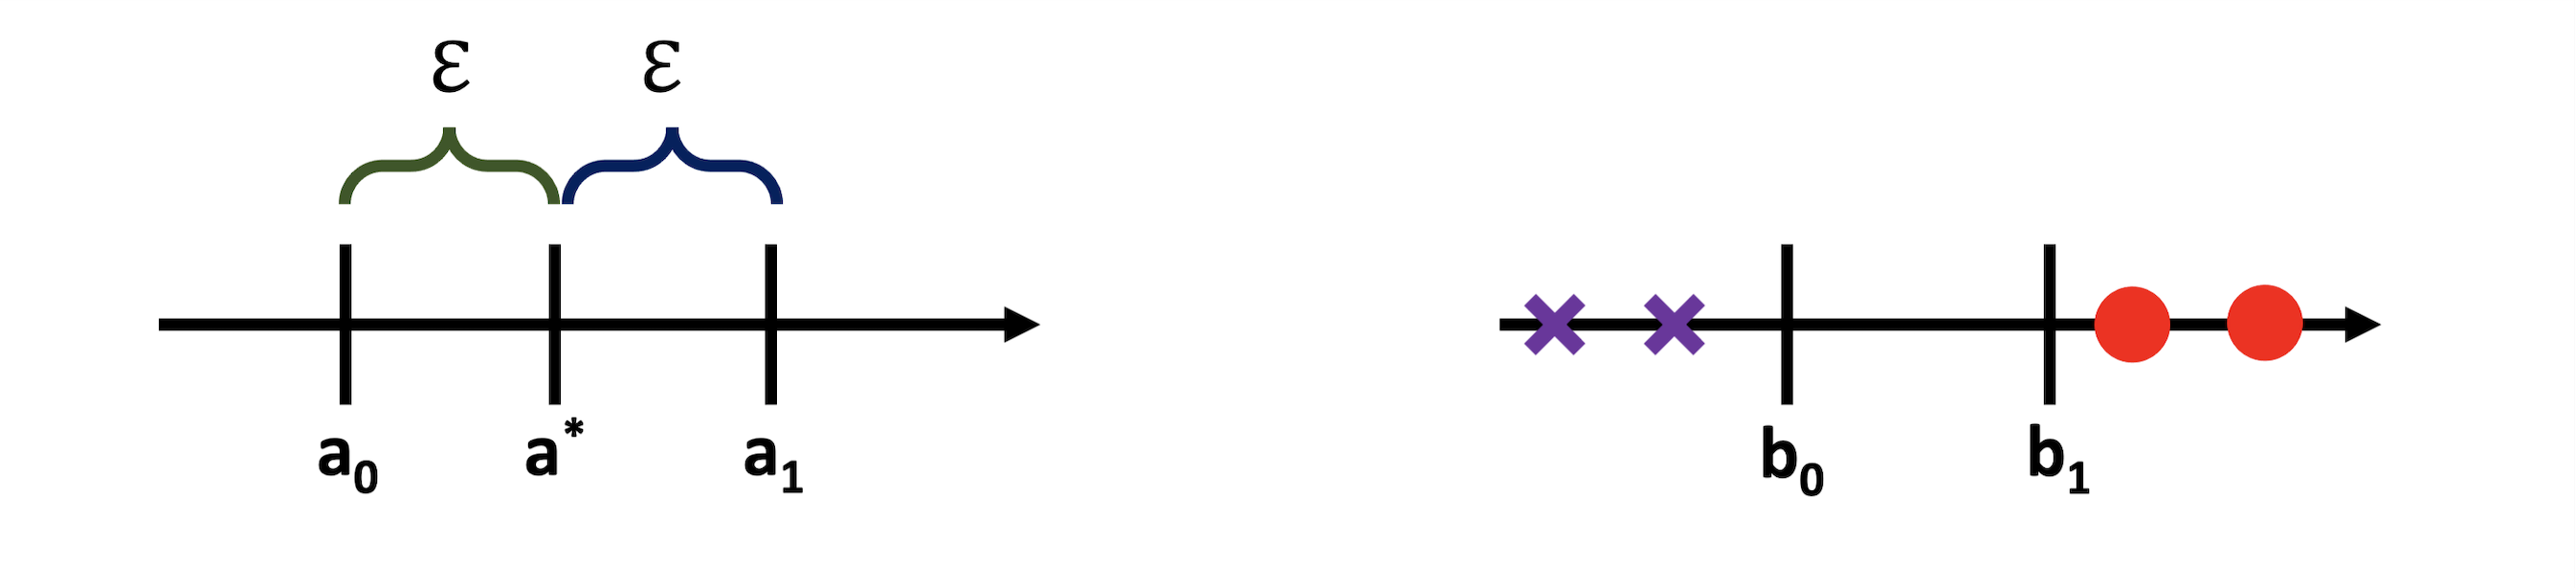
\includegraphics[width=0.8\columnwidth]{imagen09_1.png}
      \caption{{\textsf{Figuras complementarias al texto.}}  Figura de la recta numérica [izquierda] que muestra que la $a^*$ se encuentra a la mitad del intervalo $(a_0,a_1)$. Figura de la recta numérica [derecha] que muestra el comportamiento del conjunto $S$}\label{fig:imag_1}
    \end{figure}

\noindent Ahora, se tiene a $S$, un conjunto de entrenamiento tal que $b_0 = max\{ x: (x,1) \in S \}$ y $b_1 = min\{ x: (x,0) \in S \}$. Esto se puede ver reflejado en el lado derecho de la \cref{fig:imag_1}. Gracias al ERM, definamos a $h_S=h_{b_S}$ tal que $b_S \in (b_0, b_1)$. Tenemos que $\mathcal{L}(h_S) \leq \epsilon$ es suficiente para $b_0 \geq a_0$ y $b_1 \leq a_1$, ahora analizando el complemento, tenemos lo siguiente:
$$ \mathds{P}_{S \thicksim \mathcal{D}^m}(\mathcal{L}_\mathcal{D}(h_S) > \epsilon) \leq \mathds{P}_{S \thicksim \mathcal{D}^m}(b_0 < a_0 \cup b_1 > a_1) \leq \mathds{P}_{S}(b_0 < a_0) + \mathds{P}_{S}(b_1 > a_1) .$$

\noindent  Cabe mencionar que el evento $b_0 < a_0$ ocurre si todos los ejemplos en $S$ no se encuentran en $(a_0,a^*)$, por lo tanto como $m > {\frac{log(\frac{2}{\delta})}{\epsilon}}$ , se cumple lo siguiente:

$$ \mathds{P}(b_0 < a_0) = \mathds{P}(\forall (x,y) \in S, x \notin (a_0,a^*)) = (1-\epsilon)^m \leq e^{-\epsilon m} \leq \frac{\delta}{2}.$$ 

\noindent Es análogo para el caso de $b_1 > a_1$ en donde se obtiene que $\mathds{P}(b_1 > a_1) \leq \frac{\delta}{2}.$\\

\noindent \textit{Nota:} Esta solución nos muestra que entonces sí podemos aprender cuando tenemos un espacio infinito de funciones gracias al ERM.

\end{example}

\section{Dimensión VC: Vapnik-Chervonenkis}

Hasta ahorita, hemos visto que si tenemos clases finitas, entonces tenemos capacidad de aprendizaje; por otro lado, que podemos utilizar el Teorema $NFL$ para las ocasiones en las que restringimos el tamaño de $\mathcal{H}$. Ahora lo que nos interesa conocer es cómo se comporta $\mathcal{H}$ en $\C$ si no lo restringimos, además, es importante mencionar que puede suceder que el adversario escoja, dentro de la familia de distribuciones, un agente que nos perjudique para que no sea PAC aprendible.

\begin{center}
    \begin{minipage}[c]{0.7\linewidth}
      \begin{definition}[Restricción de $\mathcal{H}$ en $\C$]\label{def:ResH_C}
        Sea $\mathcal{H}$ una familia de hipótesis donde h: $\chi\rightarrow \{0, 1\}$ y sea $\C=\{C_1, ..., C_m\}$ $\subset$ $\chi$. La restricción de $\mathcal{H}$ en $\C$ tal que,
        $$ \mathcal{H}_\C = \{(h(C_1), ..., h(C_m)): h \in \mathcal{H}, C_j \in \C\}.$$
      \end{definition}
    \end{minipage}
  \end{center}
  
 \begin{center}
    \begin{minipage}[c]{0.7\linewidth}
      \begin{definition}[Fragmentación]\label{def:Frag}
        Decimos que la clase de funciones $\mathcal{H}$  fragmenta un conjunto finito $\C \subset \chi$ si $\mathcal{H}_\C$ considera todas las funciones $\C$ a \{0, 1\} tal que $\mid \mathcal{H}_\C \mid = 2^{\mid \C \mid}$.
      \end{definition}
    \end{minipage}
  \end{center}

\begin{example}
\noindent Tomando la definición de $\mathcal{H}_a$ (la familia de funciones indicadoras) y definiendo a $\C=\{C_1\}$ con $C_1 \in \R$, tenemos que:

\begin{enumerate}
	\item $a=C_1 + 1\implies h_a(C_1)=1$ 
	\item $a=C_1 - 1 \implies h_a(C_1)=0$ 
\end{enumerate}

Podemos observar que $(\mathcal{H}_a)_\C$ incluye todas las posibles funciones de $\C \rightarrow \{0,1\}$, por lo tanto, $\mathcal{H}$ fragmenta conjuntos de cardinalidad igual a 1.\\

Ahora, definiendo $\C=\{C_1, C_2\}$ con $C_1 \leq C_2$, vemos que si quisiéramos etiquetar a $C_1$ y $C_2$ de tal manera que obtengamos 0 y/o 1, vemos que no se puede debido a la restricción  $C_1 \leq C_2$, por lo tanto, $\mathcal{H}_a$ no fragmenta a $\C$ con cardinalidad igual a 2.\\
\end{example}

\begin{center}
    \begin{minipage}[c]{0.7\linewidth}
      \begin{corollary}\label{cor:FamHip}
      Sea $\mathcal{H}$ una familia de hipótesis $\chi \rightarrow \{0, 1\}$, $S$ conjunto de entrenamiento con m observaciones. Suponemos que existe $\C \subset \chi, \mid \C \mid = 2m$ y que es fragmentado por $\mathcal{H}$. Entonces $\forall$ A $\exists$ una distribución $\mathcal{D}$ sobre $\chi \times \{0, 1\}$ y un predictor $h \in \mathcal{H}$ tal que $ \mathcal{L}_\mathcal{D}(h)=0$, pero con probabilidad $\geq \frac{1}{7}$ tenemos que $ \mathcal{L}_\mathcal{D}(A(S)) \geq \frac{1}{8} $.
      \end{corollary}
    \end{minipage}
  \end{center}

\begin{center}
    \begin{minipage}[c]{0.7\linewidth}
      \begin{definition}[Dimensión Vapnik-Chervonenkis]\label{def:Dim}
      La dimensión VC de $\mathcal{H}$, $VCdim(\mathcal{H})$, es el tamaño más grande de $\C$ que puede ser fragmentado por $\mathcal{H}$.
      \end{definition}
    \end{minipage}
  \end{center}

\begin{center}
    \begin{minipage}[c]{0.7\linewidth}
      \begin{remark}\label{rem:Fragmentar}
      Si $\mathcal{H}$ puede fragmentar cualquier $\C$ $\implies$ $VCdim(\mathcal{H})=\infty$.
      \end{remark}
    \end{minipage}
  \end{center}

\begin{center}
    \begin{minipage}[c]{0.7\linewidth}
      \begin{theorem}\label{thm:DimVC1}
        Sea $\mathcal{H}$, $VCdim(\mathcal{H})=\infty$ $\implies$ $\mathcal{H}$ no es PAC.
      \end{theorem}
    \end{minipage}
  \end{center}

\section{Ejemplos de dimensión VC} 

Considerando que $VCdim(\mathcal{H})=d$, tenemos que:

\begin{enumerate}
	\item Mostrar que un conjunto $\C$,  $\mid \C \mid=d$, es fragmentado por $\mathcal{H}$.
	\item Mostrar que cualquier $\C$, $\mid \C \mid=d+1$, no es fragmentado por $\mathcal{H}$.
\end{enumerate}

\subsection{Indicadores}

\noindent Caso 1: Sea $\C = \{C_1\}$ --------------------------------------------------------------------- Sí procede \\
\noindent Caso 2: Sea $\C = \{C_1, C_2\}$ ----------------------------------------------------------------- No procede \\

Por lo tanto, $VCdim(\mathcal{H})=1$.

\subsection{Intervalos}

\noindent Sea  $\mathcal{H}_{a,b}=\{h_{a,b}: a, b \in \R, a <b\}$ tal que $h_{a,b}(x)=\mathds{1}_{[x \in (a,b)]}$. \\

\noindent Caso 1: Sea $\C = \{C_1, C_2\}$ ----------------------------------------------------------------- Sí procede \\
\noindent Caso 2: Sea $\C = \{C_1, C_2, C_3\}$ ------------------------------------------------------------ No procede \\

Vemos que sin pérdida de generalidad, considerando $C_1 \leq C_2 \leq C_3$, se presenta un problema ya que no se puede etiquetar con solo 0 y 1, por ejemplo, no se puede $1 \leq 0 \leq 1$. Por lo tanto $VCdim(\mathcal{H}_{a,b})=2$.

\subsection{Rectángulos}

\noindent Sea  $\mathcal{H}=\{h_{\theta}: \theta = (a_1, a_2, b_1, b_2), a_1 \leq a_2, b_1 \leq b_2 \}$. 
$$h_\theta(x_1, x_2) = \left\{ \begin{array}{lcc}
             1 &   si  & x_1 \in (a_1, a_2), x_2 \in (b_1, b_2) \\
             \\ 0 &  en & c.o.c.
             \end{array} \right.$$
En la \cref{fig:imag_2} podemos observar que $VCdim(\mathcal{H}_{a,b})=4$. Del lado izquierdo está el caso de 4 puntos (que Sí procede), mientras que del lado derecho es el caso de 5 puntos (que No procede).

   \begin{figure}[h!]
      \centering
      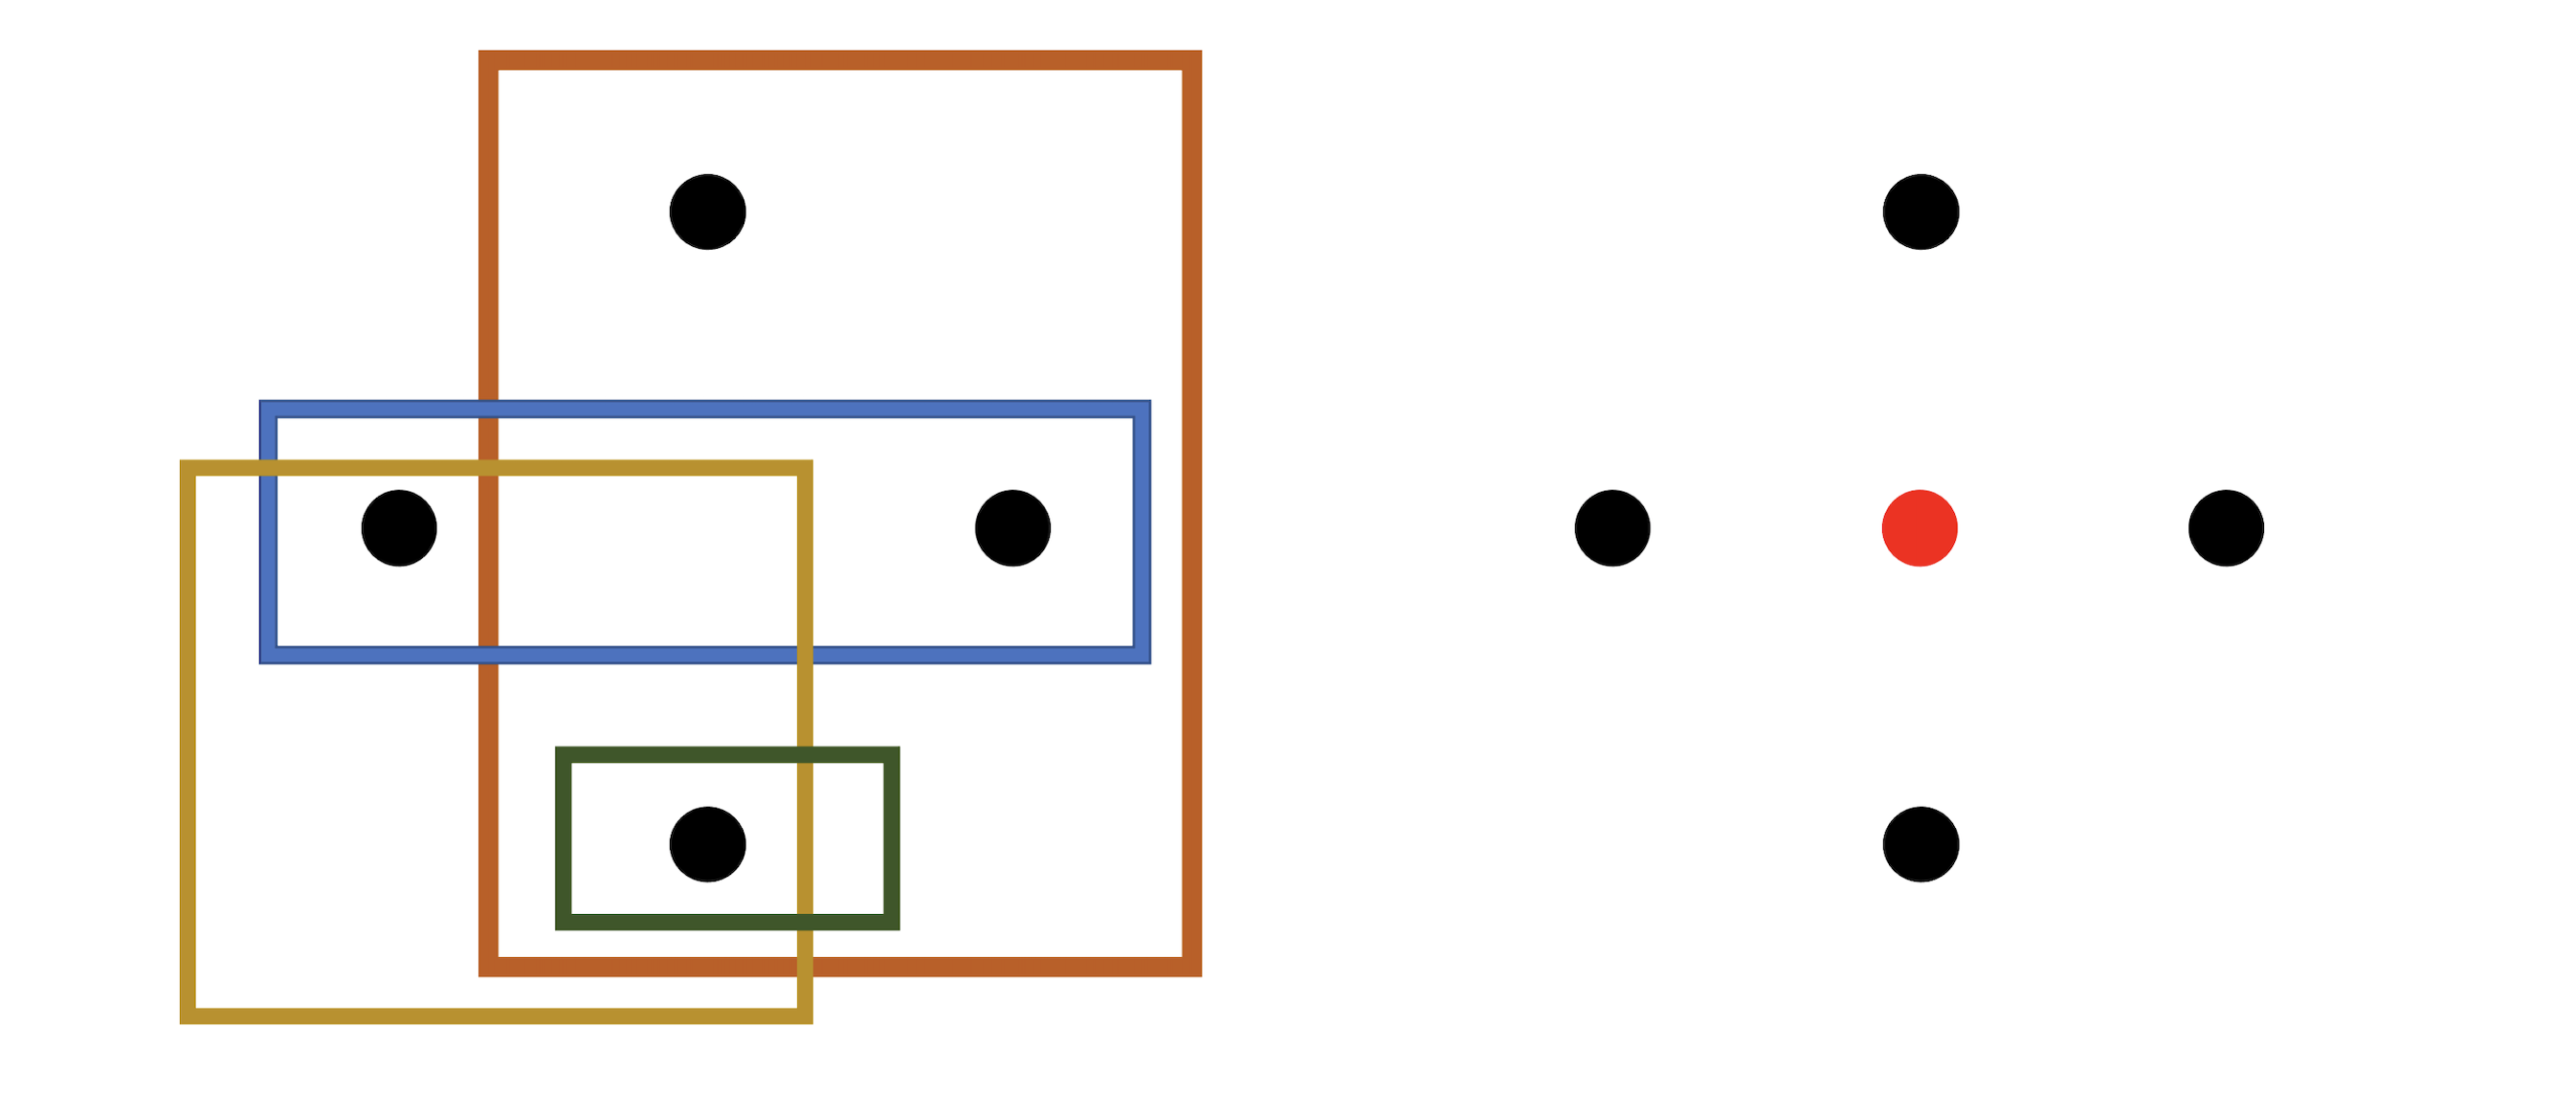
\includegraphics[width=0.7\columnwidth]{imagen09_2.png}
      \caption{{\textsf{Figuras de casos para rectángulos.}}  Figura de etiquetados de puntos [izquierda] que se muestra que sí pueden ser etiquetados sin ningún problema. Figura de etiquetados [derecha] que muestra un problema porque si suponemos que el punto rojo es negativo, no hay manera de poder etiquetarlos correctamente.} \label{fig:imag_2}
    \end{figure}


\subsection{Clases finitas}

Sea $\mathcal{H}$, clase finita, tal que $\forall$ $\C \subset \mid \mathcal{H}_\C \mid \leq \mid \mathcal{H} \mid$ y por lo tanto $\C$ no es fragmentado por $\mathcal{H}$ si $\mid \mathcal{H} \mid < 2^{\mid \C \mid} \implies VCdim(\mathcal{H}) \leq log_2(\mid \mathcal{H} \mid)$, es decir, está acotado, sin embargo, dicha cota en general se considera como mala, ya que la $VCdim(\mathcal{H})$ de una clase de hipótesis finita puede ser significativamente más pequeña que $log_2(\mid \mathcal{H} \mid)$.

\section{El Teorema Fundamental de Aprendizaje Estadístico}

\begin{center}
    \begin{minipage}[c]{0.7\linewidth}
      \begin{theorem}[Teorema Fundamental de Aprendizaje Estadístico]\label{th:TFAE}
      Sea $\mathcal{H}$ tal que $h \in \mathcal{H}$ h:$\chi \rightarrow \{0, 1\}$ y consideramos la pérdida 0-1. Entonces los siguientes enunciados son equivalentes:
\begin{enumerate}
	\item $\mathcal{H}$ tiene la propiedad de convergencia uniforme.
	\item ERM es capaz de generar aprendizaje PAC agnóstico con $\mathcal{H}$.
	\item $\mathcal{H}$ es PAC agnóstico.
	\item $\mathcal{H}$ es PAC.
	\item ERM es capaz de generar aprendizaje PAC.
	\item $\mathcal{H}$ tiene $VCdim(\mathcal{H})<\infty$.
\end{enumerate}
      \end{theorem}
    \end{minipage}
  \end{center}

%>>>>>> END OF YOUR CONTENT

\end{document}
